\documentclass[border=10pt]{standalone}
\usepackage{pgfplots}
\pgfplotsset{width=7cm, compat=1.8}
\usepackage{pgfplotstable}
\renewcommand*{\familydefault}{\sfdefault}
\usepackage{sfmath}

\begin{document}

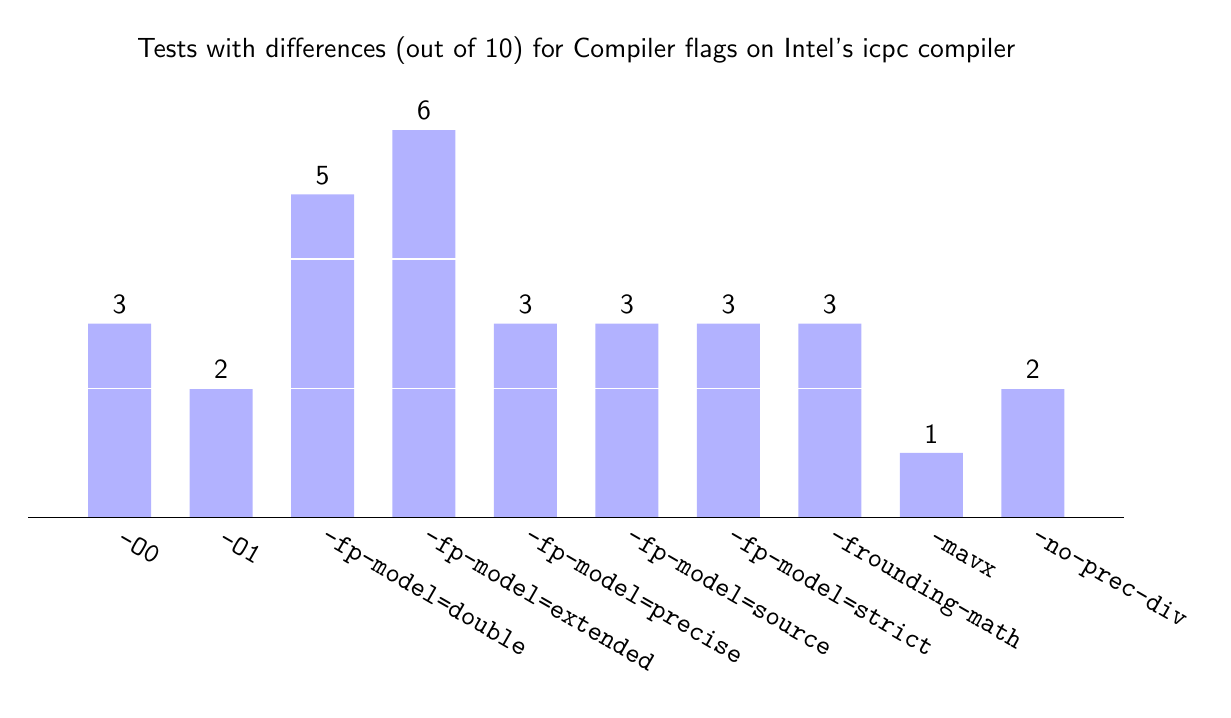
\begin{tikzpicture}
  \centering
  \begin{axis}[
    ybar,
    axis on top,
    title={Tests with differences (out of 10) for Compiler flags on Intel's icpc compiler},
    height=7cm,
    width=15.5cm,
    bar width=0.8cm,
    ymajorgrids,
    tick align=inside,
    major grid style={draw=white},
    ymin=0,
    axis x line*=bottom,
    axis y line*=right,
    y axis line style={opacity=0},
    yticklabel style={opacity=0},
    tickwidth=0pt,
    enlarge x limits=true,
    symbolic x coords={
      -O0,
      -O1,
      -fp-model=double,
      -fp-model=extended,
      -fp-model=precise,
      -fp-model=source,
      -fp-model=strict,
      -frounding-math,
      -mavx,
      -no-prec-div,
      },
    xtick=data,
    xticklabel style={ rotate=-30, anchor=west, yshift=-0.2cm , font=\ttfamily },
    nodes near coords={
      \pgfmathprintnumber[precision=0]{\pgfplotspointmeta}
      },
    ]
    \addplot [draw=none, fill=blue!30] coordinates {
      (-fp-model=extended, 6)
      (-fp-model=double,   5)
      (-fp-model=source,   3)
      (-fp-model=strict,   3)
      (-frounding-math,    3)
      (-O0,                3)
      (-fp-model=precise,  3)
      (-no-prec-div,       2)
      (-O1,                2)
      (-mavx,              1)
      };
  \end{axis}
  This is compared with having no command-line arguments at all (except
  -mlong-double-80 which was used for all runs)
\end{tikzpicture}



%\begin{tikzpicture}
%  \centering
%  \begin{axis}[
%    ybar,
%    axis on top,
%    title={Cumulative Progress of Works},
%    height=7cm,
%    width=15.5cm,
%    bar width=0.4cm,
%    ymajorgrids,
%    tick align=inside,
%    major grid style={draw=white},
%    enlarge y limits={value=.1,upper},
%    ymin=0,
%    ymax=100,
%    axis x line*=bottom,
%    axis y line*=right,
%    y axis line style={opacity=0},
%    tickwidth=0pt,
%    enlarge x limits=true,
%    legend style={
%      at={(0.5,-0.2)},
%      anchor=north,
%      legend columns=-1,
%      /tikz/every even column/.append style={column sep=0.5cm}
%      },
%    ylabel={Percentage (\%)},
%    symbolic x coords={
%      Sep-11,
%      Oct-11,
%      Nov-11,
%      Dec-11,
%      Jan-12,
%      Feb-12,
%      Mar-12,
%      Apr-12,
%      },
%    xtick=data,
%    nodes near coords={
%      \pgfmathprintnumber[precision=0]{\pgfplotspointmeta}
%      },
%    ]
%    \addplot [draw=none, fill=blue!30] coordinates {
%      (Sep-11, 75.4064)
%      (Oct-11, 72.7961)
%      (Nov-11, 94.4597)
%      (Dec-11, 66.6786)
%      (Jan-12, 67.5600)
%      (Feb-12, 88.2339)
%      (Mar-12, 78.6138)
%      (Apr-12, 58.9129)
%      };
%   \addplot [draw=none,fill=red!30] coordinates {
%      (Sep-11, 75.4064)
%      (Oct-11, 89.7961)
%      (Nov-11, 94.4597)
%      (Dec-11, 76.6786)
%      (Jan-12, 77.5600)
%      (Feb-12, 78.2339)
%      (Mar-12, 88.6138)
%      (Apr-12, 78.9129) };
%   \addplot [draw=none, fill=green!30] coordinates {
%      (Sep-11, 75.4064)
%      (Oct-11, 89.7961)
%      (Nov-11, 94.4597)
%      (Dec-11, 76.6786)
%      (Jan-12, 77.5600)
%      (Feb-12, 78.2339)
%      (Mar-12, 88.6138)
%      (Apr-12, 78.9129) };
%
%    \legend{First Fix,Second Fix,Third Fix}
%  \end{axis}
%\end{tikzpicture}


\end{document}
